% 3DCNN %% Video related 1.5 page
\subsection{3D-CNN and RNN based methods}
\label{subsec: 3D-CNN and RNN based methods}
The standard two-dimensional convolution uses a two-dimensional kernel filter on each channel, and only two-dimensional features can be extracted.
\citet{tran2015learning} reviewed many previous 3-dimensional convolutional networks (3D-CNN) and highlighted relevant applications on spatiotemporal features in video dataset.
As shown in Figure \ref{fig:2-2dcnn-3dcnn}, 2D convolutional kernel filters are expanded to 3D and allow them running on multiple channels simultaneously.
3D-CNN is widely used in tasks that process multiple images at the same time, such as medical computed tomography (CT) scan data and video data.

\begin{figure}[!ht]
    \centering
    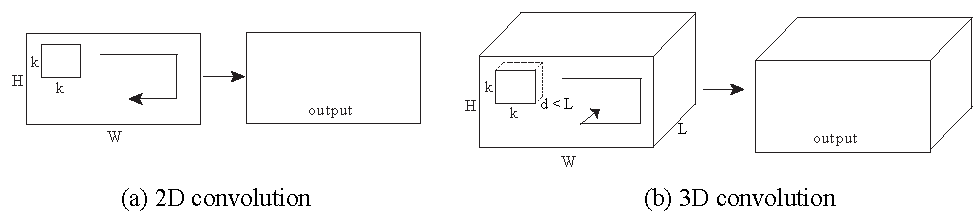
\includegraphics[width=\textwidth]{literature/imgs/2-2dcnn-3dcnn.pdf}
    \caption{2D convolution and 3D convolution \cite{tran2015learning}}
    \label{fig:2-2dcnn-3dcnn}
\end{figure}

The difference between the proposed 3D convolution and the multi-channel 2D convolution is that the 3D convolution uses weight-sharing kernel filters, while the multi-channel 2D convolutional kernel filters have different weights for each channel and ignore adjacent channels in computation.

Back to 2011, \citet{baccouche2011sequential} firstly applied a composed architecture of 3D convolution and RNN to the human action recognition task.
In this work, 3D convolution is firstly used for learning spatiotemporal features automatically, followed by an RNN `` to classify each sequence considering the temporal evolution of the learned features for each timestep'', said by \citet{baccouche2011sequential}.
The researchers also spotted the performance drawback of the RNN and will investigate the possibility of using a single-step model in future work.

One year after, \citet{ji20123d} proposed a human action recognition model composed purely of convolutional operations. %, as shown in Figure \ref{fig:ext-2-3dcnn-har}.
The premature network design is shallow and does not use residual connections, which are very similar in architecture to LeNet, consisting of multiple convolutional layers and pooling layers. In addition, they add some designed features (optical flow fields in many directions) to input, which is not an end-to-end trainable network.

% \begin{figure}[!ht]
%     \centering
%     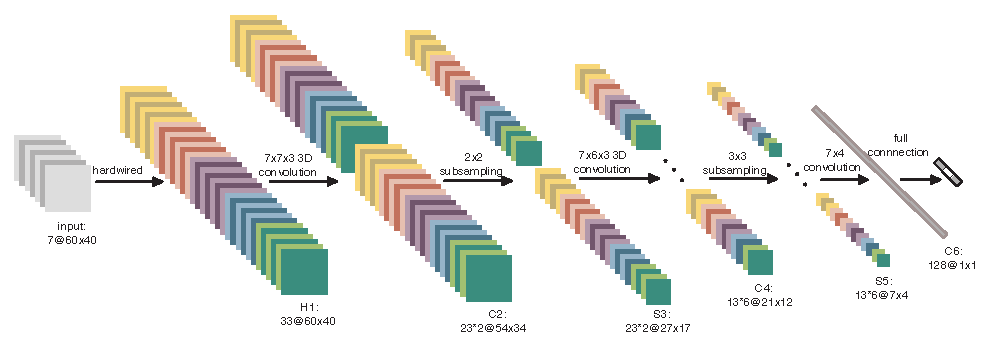
\includegraphics[width=\textwidth]{literature/imgs/ext-2-3dcnn-har.pdf}
%     \caption{A 3D-CNN model for human action recognition \cite{ji20123d}}
%     \label{fig:ext-2-3dcnn-har}
% \end{figure}

After several years of development, \citet{tran2015learning} proposed model Convolutional 3D (C3D) that achieved the state-of-the-art in video tasks in 2015.
This model does not involve the input of additional handcrafted features at all, but it also exposes some weaknesses of the 3D convolution.
For example, 3D-CNN cannot use pre-trained results from 2D images, such as ImageNet.
Also, the network has too many parameters, which is prone to over-fitting in the case of using an insufficient amount of video training data.

To overcome the weaknesses of using CNN or RNN individually, \citet{simonyan2014twostream} proposed a Two-Stream network.
The network consists of a spatial flow focused on each image frame and a temporal flow focused on the calculated optical flow.
Based on the idea of using the Two-Stream network, \citet{feichtenhofer2016convolutional} pointed out that the fusion process in the last Softmax layer caused losses and 3D convolution can perfectly fuse the spatiotemporal information in the convolutional layers.

In 2018, \citet{carreira2018quo} summarised the previous research on different methods used in the field of action recognition, which is also discussed in this subsection, namely ConvNet+LSTM (CNN+RNN), 3D ConvNets (3D-CNN) and Two-Stream network.
Based on these previous ideas, Inflated Two-Stream 3D ConvNets (I3D) is proposed and achieved good results on both HMDB-51 and UCF-101 data sets.